%%%%%%%%%%%%%%%%%%%%%%%%%%%%%%%%%%%%%%%%%%%%%%%%%%%%%%%%%%%%%%%%%%%%%%
% Overleaf (WriteLaTeX) Example: Molecular Chemistry Presentation
%
% Source: http://www.overleaf.com
%
% In these slides we show how Overleaf can be used with standard 
% chemistry packages to easily create professional presentations.
% 
% Feel free to distribute this example, but please keep the referral
% to overleaf.com
% 
%%%%%%%%%%%%%%%%%%%%%%%%%%%%%%%%%%%%%%%%%%%%%%%%%%%%%%%%%%%%%%%%%%%%%%
% How to use Overleaf: 
%
% You edit the source code here on the left, and the preview on the
% right shows you the result within a few seconds.
%
% Bookmark this page and share the URL with your co-authors. They can
% edit at the same time!
%
% You can upload figures, bibliographies, custom classes and
% styles using the files menu.
%
% If you're new to LaTeX, the wikibook is a great place to start:
% http://en.wikibooks.org/wiki/LaTeX
%
%%%%%%%%%%%%%%%%%%%%%%%%%%%%%%%%%%%%%%%%%%%%%%%%%%%%%%%%%%%%%%%%%%%%%%

\documentclass{beamer}

% For more themes, color themes and font themes, see:
% http://deic.uab.es/~iblanes/beamer_gallery/index_by_theme.html
%
\mode<presentation>
{
  \usetheme{Madrid}       % or try default, Darmstadt, Warsaw, ...
  \usecolortheme{default} % or try albatross, beaver, crane, ...
  \usefonttheme{serif}    % or try default, structurebold, ...
  \setbeamertemplate{navigation symbols}{}
  \setbeamertemplate{caption}[numbered]
} 

\usepackage[english]{babel}
\usepackage[utf8x]{inputenc}
\usepackage{chemfig}
\usepackage[version=3]{mhchem}

% On Overleaf, these lines give you sharper preview images.
% You might want to `comment them out before you export, though.
\usepackage{pgfpages}
\pgfpagesuselayout{resize to}[%
  physical paper width=8in, physical paper height=6in]

%==================================
\usepackage{subfigure}
%==================================

% Here's where the presentation starts, with the info for the title slide
\title[My Computer Graphics Background]{A short presentation on my background in computer graphics}
\author{M. Mostajab}
\institute{www.mmostajab.com}
\date{\today}

\begin{document}

\begin{frame}
  \titlepage
\end{frame}

% These three lines create an automatically generated table of contents.
\begin{frame}{Outline}
  \tableofcontents
\end{frame}

\section{Introduction}

\begin{frame}{About Me...}
	\begin{tikzpicture}[overlay, remember picture]
		\node[anchor=north east, xshift=-30pt,yshift=-55pt]
		at(current page.north east){
			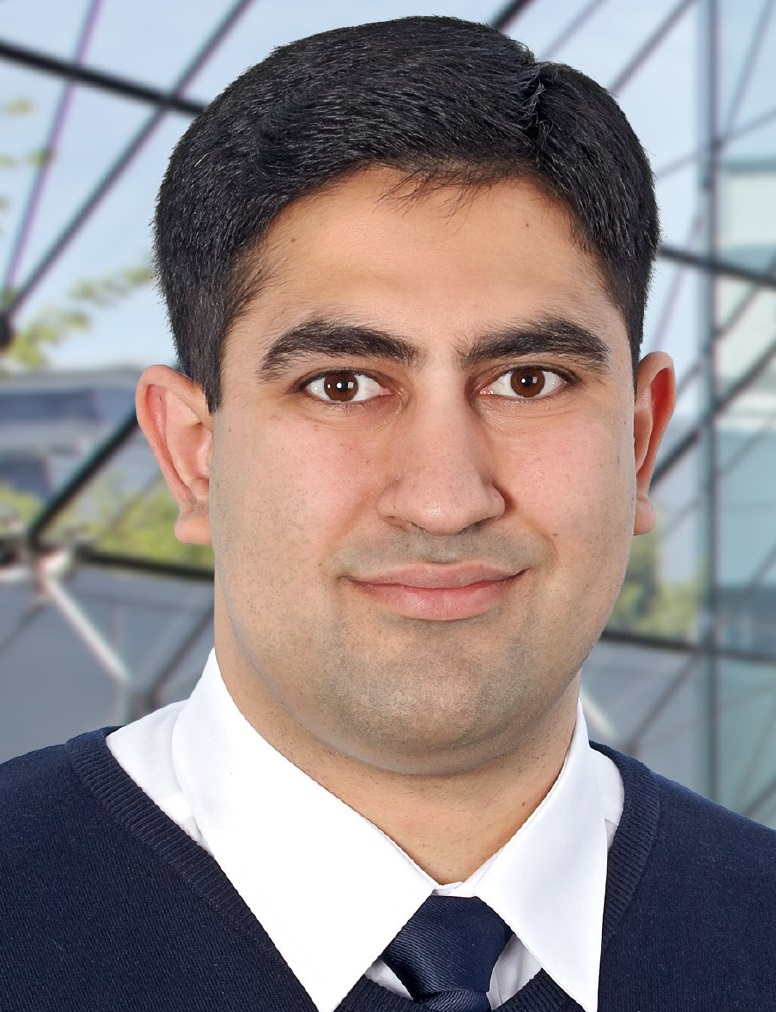
\includegraphics[width=30mm]{figures/photo.jpg}
		};
	\end{tikzpicture}

	\begin{itemize}
		\item My name is \textbf{Morteza Mostajab} \cite{Barringer:2014:DRS:2601097.2601222} \cite{pgs.20141257}
		\item Bachelor studies:\\ \textit{Hamedan University of Technology, Iran}
		\item Maseter studies:\\ \textit{Technische Universit{\"a}t M{\"unchen}}
		\item Present:\\ \textit{Researcher at Fraunhofer IGD, Darmstadt}
		\item Research interests:\\
		    \textit{Real-time physically-based rendering} \\
			\textit{(Rasterization-based or Ray-tracing)}\\
			\textit{Virtual reality}\\
			\textit{Computer graphics and visualization}\\
			\textit{Game Programming}
		   
	\end{itemize}
\end{frame}

\begin{frame}{Inspiration}
	
	\begin{itemize}
		\item Games, Animations, Movies with Special Effects,...
			\begin{figure}
			\centering
			\subfigure[Last Ninja 3]{
				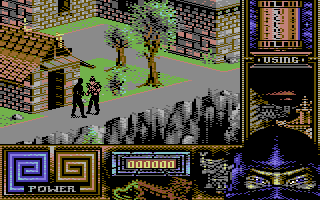
\includegraphics[width=0.19\linewidth]{figures/LastNinja.png}
			}
			%\subfigure[Warcraft 2]{
			%	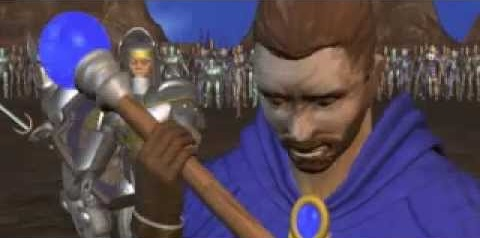
\includegraphics[width=0.2\linewidth]{figures/warcraft2.jpg}
			%}
			\subfigure[Gears of War]{
				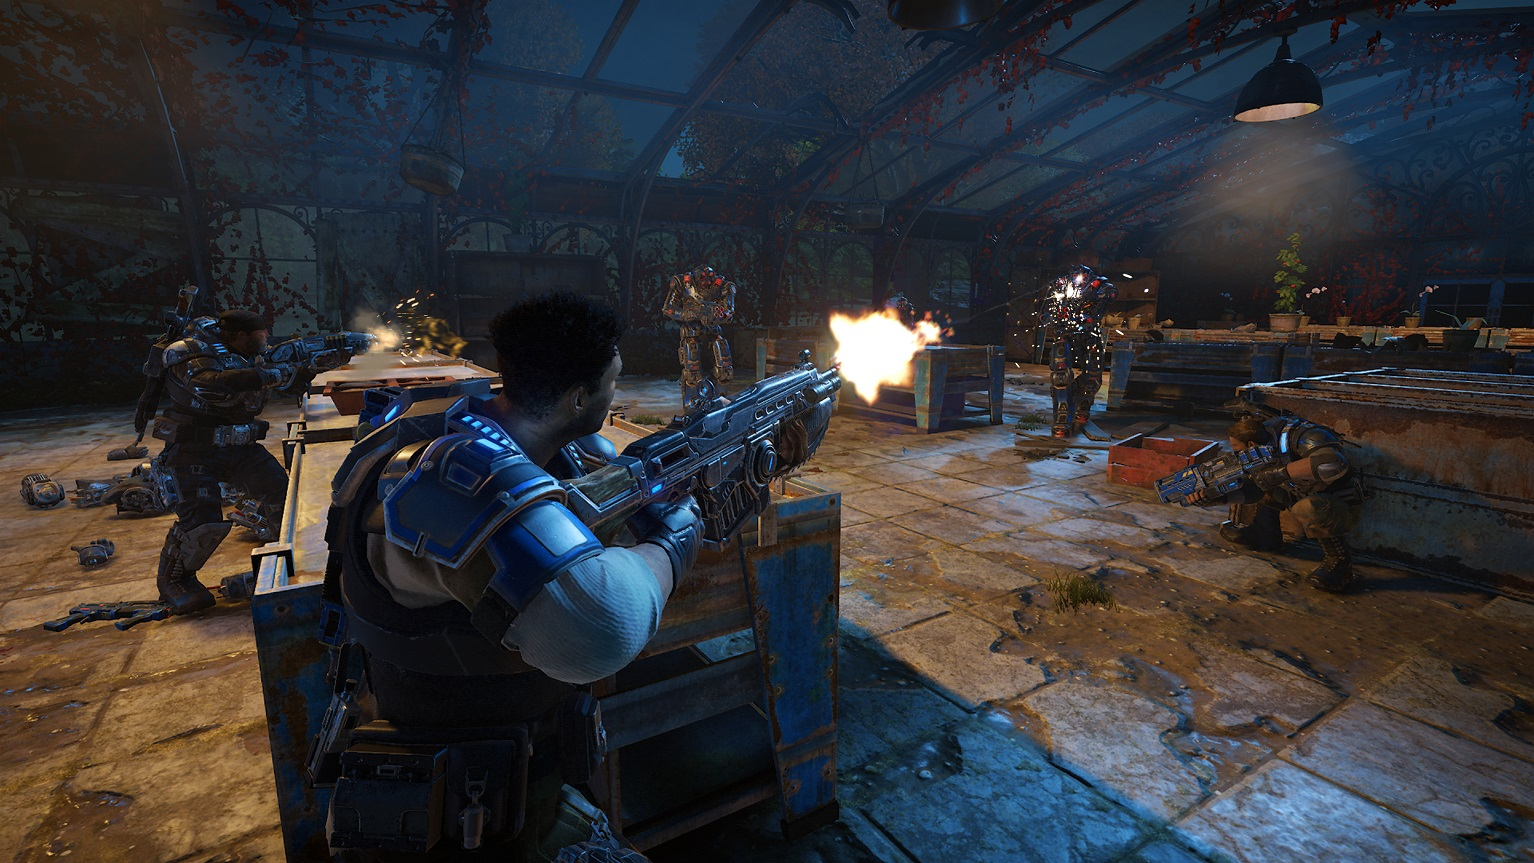
\includegraphics[width=0.21\linewidth]{figures/geow.jpg}
			}
			\subfigure[Ratatouille]{
				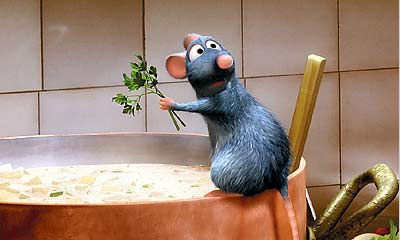
\includegraphics[width=0.20\linewidth]{figures/Ratatouille.jpg}
			}
			\subfigure[The lord of the rings]{
				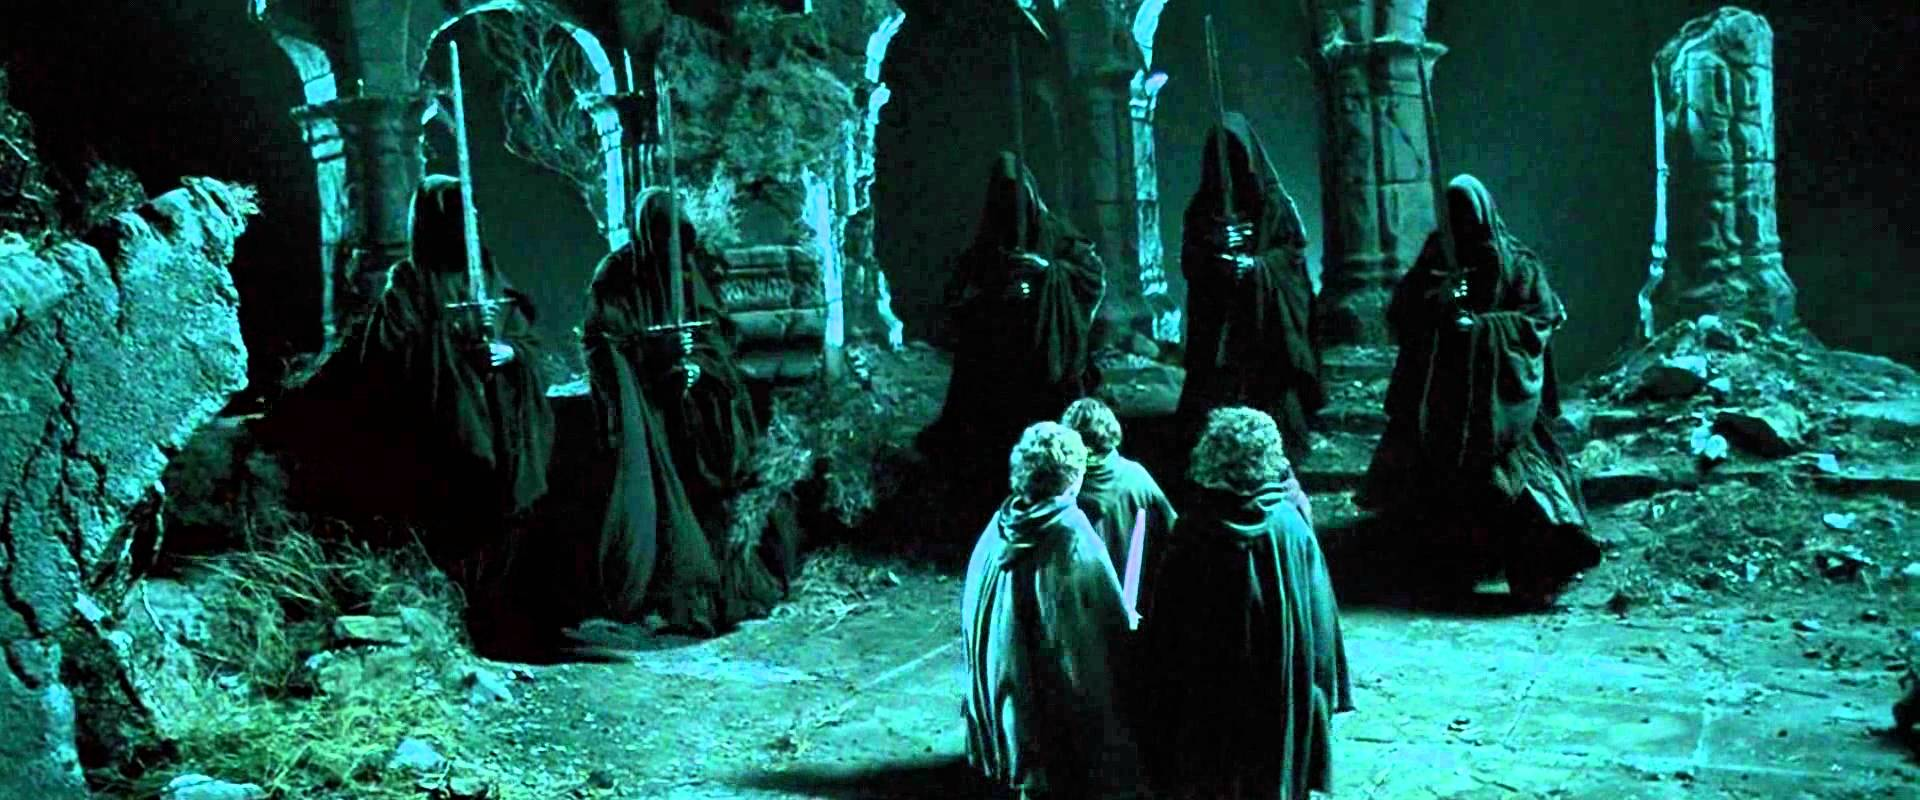
\includegraphics[width=0.29\linewidth]{figures/lotr.jpg}
			}		
		\end{figure}
	  \item My firsts...
		  \begin{figure}
			\centering
			\subfigure[First Computer]{
				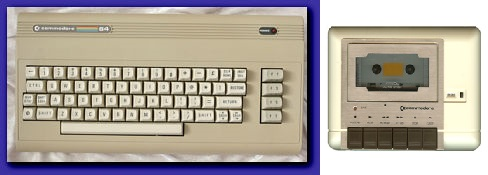
\includegraphics[height=0.2\textheight]{figures/commodore.jpg}
			}
			\subfigure[First IBM compatiable PC]{
				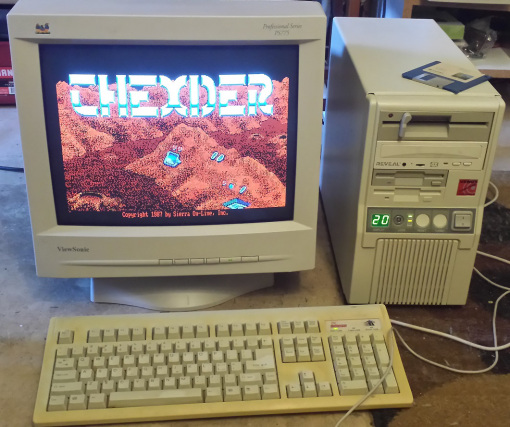
\includegraphics[height=0.2\textheight]{figures/PC286.jpg}
			}
			\subfigure[First Console (Atari 2600)]{
				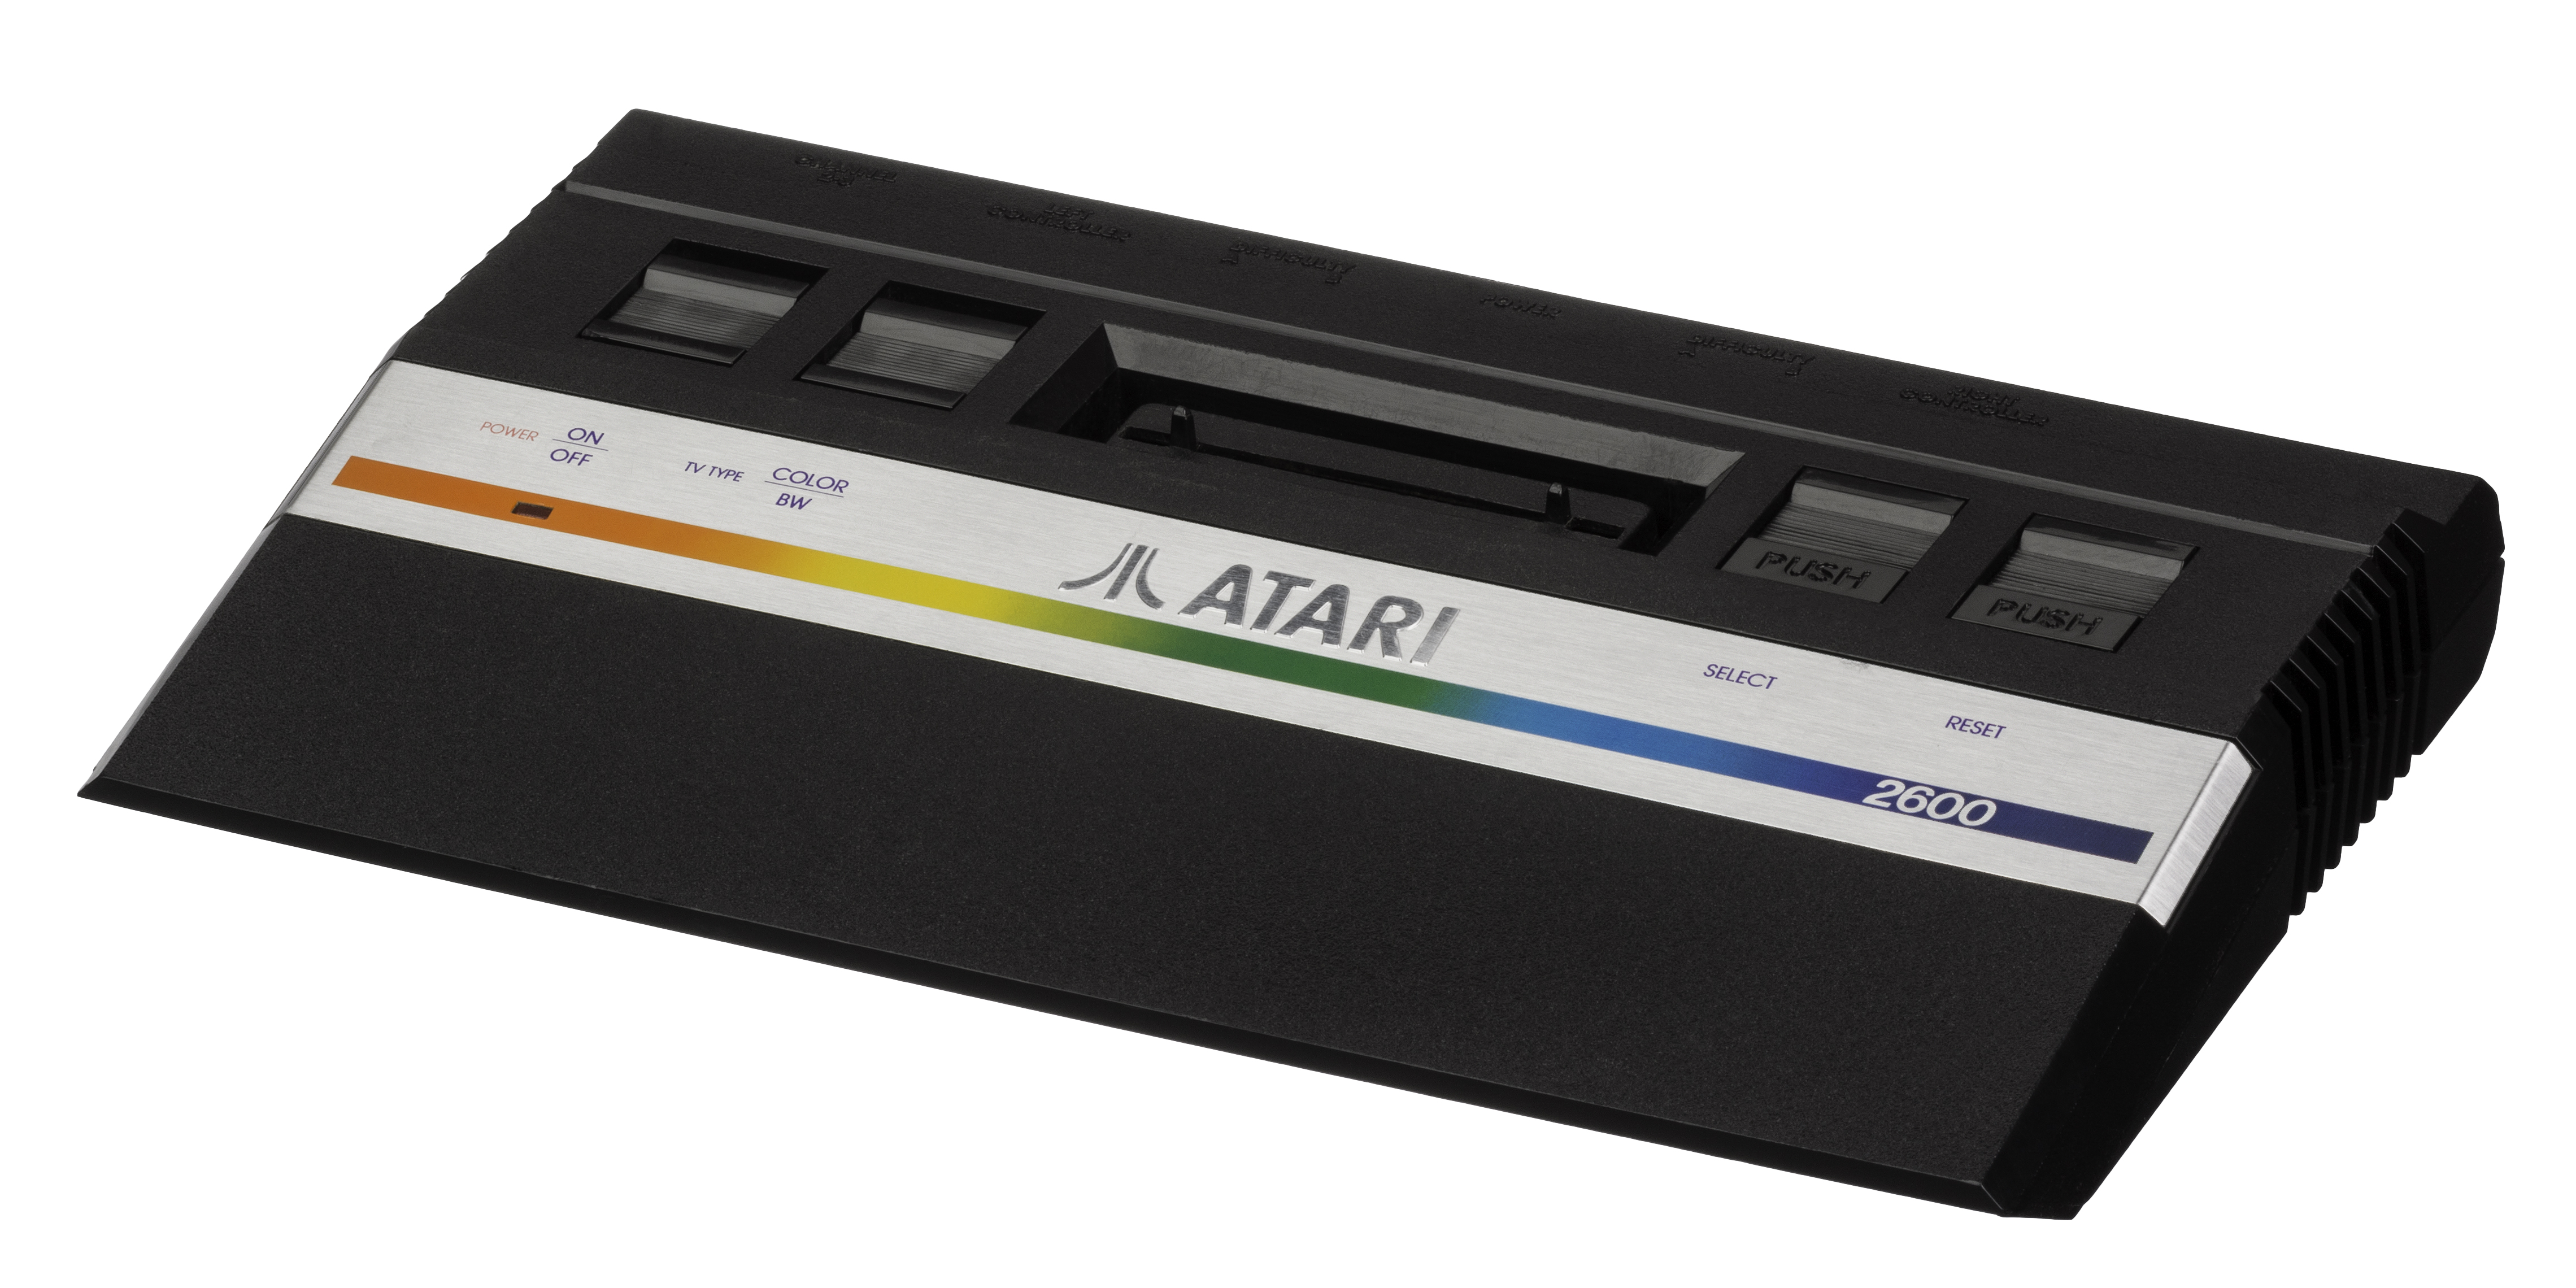
\includegraphics[height=0.15\textheight]{figures/atari2600.jpg}
			}
       	  \end{figure} 
	\end{itemize}
\end{frame}

\section{Master Thesis}

\section{Ray tracing revisited for rendering CSG models consisting of higher order primitives}

\begin{frame}{Higher order primitives}
	
	\begin{figure}[ht!]
		\centering
		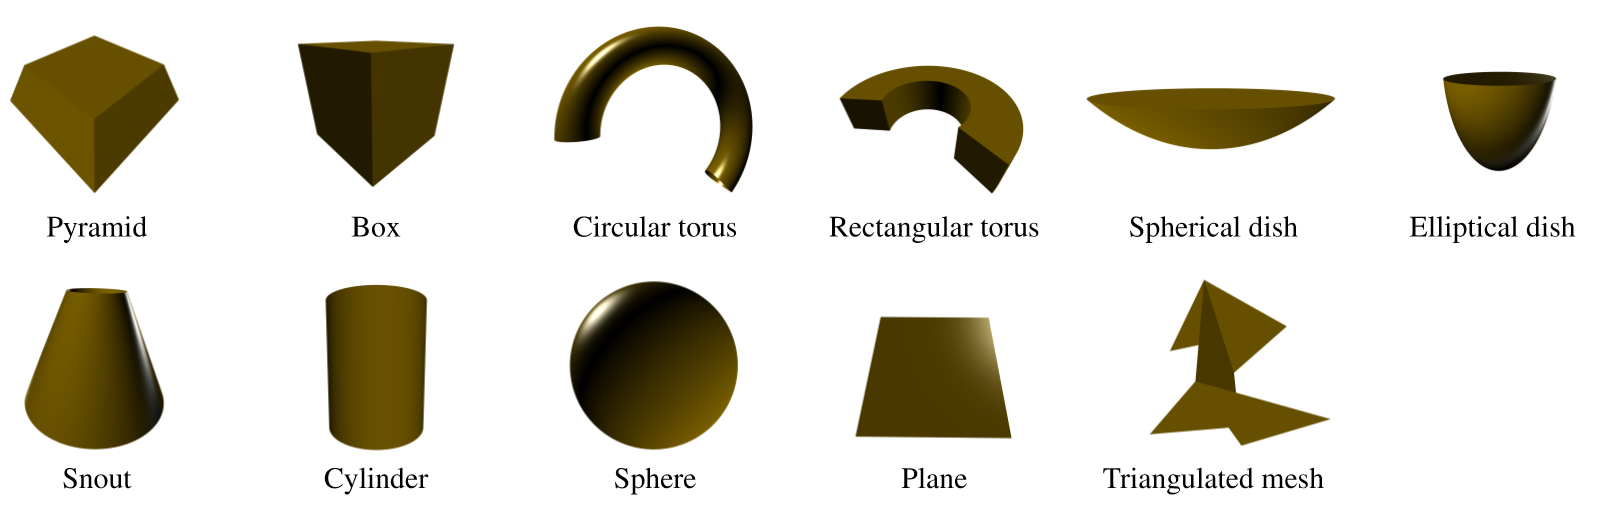
\includegraphics[width=0.9\linewidth]{figures/hops.png}
	\end{figure}
\end{frame}

\begin{frame}[allowframebreaks]
	\frametitle{References}
	\bibliographystyle{amsalpha}
	\bibliography{bibliography}
\end{frame}

\end{document}